% !TeX spellcheck = en_GB
% !TeX encoding = UTF-8
\documentclass[8pt]{beamer}

\usepackage[utf8]{inputenc}                                                     
 \usetheme[block=fill,progressbar=foot,background=light]{metropolis}                                                               
%  \usecolortheme{crane}                                                       
  %\useinnertheme{circles}                                                         
  \usepackage[english]{babel}                                                     
  \usepackage{csquotes}                                                           
  \usepackage[T1]{fontenc}                                                        
  \usepackage{booktabs}                                                       \usepackage{pgfgantt}
  \usepackage{pifont}
  \usepackage{adfbullets}
  \usepackage{enumitem}
  \usepackage{amsmath}   
  \usepackage{tikz}
  \usepackage{amssymb}
  \usepackage{amsfonts}
  \usepackage{mathrsfs}   
  \usepackage{graphicx}
  \usepackage{adjustbox}
  \usepackage{varioref}
  \usepackage{probsoln}
  \usepackage{attachfile2}
  \usepackage{pgfplots}
\pgfplotsset{compat=newest}
  \usepackage[style=authoryear,backref=true]{biblatex}
 \usepackage[]{hyperref} 
  \graphicspath{{Graphics/}}
  \usepackage{multirow,array}
  \addbibresource{../Everything.bib}
  \usepackage{colortbl}
  \definecolor{aa}{RGB}{255, 124, 0}
  \definecolor{cc}{RGB}{230, 230, 230}    
  %\setbeamercolor{palette tertiary}{fg=aa,bg=cc}
  %\setbeamercolor{structure}{fg=cc}
  %\setbeamercolor{alerted text}{fg=red}
  
  %Information to be included in the title page:
  
  \usebackgroundtemplate{%
  \tikz[overlay,remember picture]{\node[scale=80,opacity=0.03, at=(current page.south east)] {\adfbullet{9}};}}
  
  \author[]{T. Bretschneider}
  
  \date[\today]{\today}

\usepackage{comment}
\usepackage{varwidth}

\newcommand{\mat}[4]{\left(\begin{array}{cc} #1 & #2 \\ #3 & #4 \\ \end{array}\right)}
\newcommand{\Q}{\mathbb{Q}}
\newcommand{\R}{\mathbb{R}}
\newcommand{\Z}{\mathbb{Z}}
\newcommand{\sol}[2][+]{
	\tikz[baseline]{\node[color=aa,fill=cc,rectangle,draw,anchor=base] {  {\onslide<#1->{#2}}  };}
}

\usetikzlibrary{positioning}
\usetikzlibrary{tikzmark}
\usetikzlibrary{shadings}
\usetikzlibrary{through}


\def\height{0.8cm}
\def\width{1.2cm}

		\newcommand{\keynode}[6]{\node[minimum height=\height,minimum width=\width,draw,rectangle,color=aa,fill=cc] (#3) at (#1,#2) {};
	\node[rectangle,minimum height=\height/2,minimum width=\width,above,color=aa] at (#3) {#3};
	\node[draw,rectangle,minimum height=\height/2,minimum width=\width/3,below,color=aa,fill=cc,inner sep =0cm] at (#3) {\footnotesize#4};
	\node[draw,rectangle,minimum height=\height/2,minimum width=\width/3,below,xshift=\height/2,color=aa,fill=cc,inner sep=0cm] at (#3) {\footnotesize#5};
	\node[draw,rectangle,minimum height=\height/2,minimum width=\width/3,below,xshift=-\height/2,color=aa,fill=cc,inner sep=0cm] at (#3) {\footnotesize#6}; }

\newenvironment{gantt}[3]{\begin{ganttchart}[#1,bar height=.6,bar top shift=.2,title/.style=  {draw=none},y unit chart=0.6cm,y unit title = 0.6cm,include title in canvas=false,group/.append style={draw=black,dashed},bar/.append style={fill=aa},inline,hgrid=true,Float1/.style={bar/.append style={fill=none,dashed},bar height=.8,bar top shift=0.1}]{#2}{#3}}{\end{ganttchart}}

\newenvironment{nicetable}[1]{\setlength\arrayrulewidth{0.5mm}
			\arrayrulecolor{white}
			\begin{tabular}{#1}}{\end{tabular}}
		
\setlist[itemize,1]{label={\color{aa}\huge\adfbullet{9}}}
\setlist[itemize, 2]{label={\color{aa}\large\adfbullet{9}}}

\newcommand\reshist{}
\def\reshist(#1)#2(#3)#4(#5)%
{\draw (axis cs:#1) rectangle (axis cs:#3) node [midway] {#5};}






\usepackage{colortbl}

\usetikzlibrary{intersections}

\title[Discrete]{{\color{aa}\Huge\adfbullet{9}}AL FM Discrete}
\subtitle{Linear Programming: Simplex Algorithm, \textattachfile{LinearProgrammingSimplexAlgorithm.tex}{(TeX)}}

\begin{document}

\setlength{\abovedisplayskip}{0pt}
\setlength{\belowdisplayskip}{0pt}
\setlength{\abovedisplayshortskip}{0pt}
\setlength{\belowdisplayshortskip}{0pt}


\frame{\titlepage}

\begin{frame}{Overview}
	We have already seen that when we have a linear programming problem with two variables
we can represent the feasible region on a 2D graph and then find the optimal solution (which
will usually occur at a corner of the feasible region).

In theory, we could develop this idea with more variables but the problem is that there
would need to be an axis for each variable and therefore the graph would no longer be 2D.

\begin{definition}
	Instead we use an algorithmic method which involves starting at a vertex of the feasible
region and then making improvements until we find an optimal solution.
\end{definition}
\centering
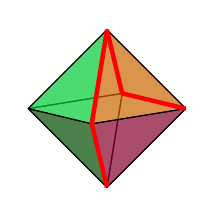
\begin{tikzpicture}[line join=bevel,z=-5.5]
\coordinate (A1) at (0,0,-1);
\coordinate (A2) at (-1,0,0);
\coordinate (A3) at (0,0,1);
\coordinate (A4) at (1,0,0);
\coordinate (B1) at (0,1,0);
\coordinate (C1) at (0,-1,0);

\draw (A1) -- (A2) -- (B1) -- cycle;
\draw (A4) -- (A1) -- (B1) -- cycle;
\draw (A1) -- (A2) -- (C1) -- cycle;
\draw (A4) -- (A1) -- (C1) -- cycle;
\draw [fill opacity=0.7,fill=green!80!blue] (A2) -- (A3) -- (B1) -- cycle;
\draw [fill opacity=0.7,fill=orange!80!black] (A3) -- (A4) -- (B1) -- cycle;
\draw [fill opacity=0.7,fill=green!30!black] (A2) -- (A3) -- (C1) -- cycle;
\draw [fill opacity=0.7,fill=purple!70!black] (A3) -- (A4) -- (C1) -- cycle;
\draw[color=red,ultra thick,yshift=0.01cm,xshift=0.01cm] (C1) -- (A3) -- (B1) -- (A1) -- (A4);
\end{tikzpicture}
\end{frame}

\begin{frame}[shrink=10]{Simplex Algorithm: Slack Variables}
	To start with we shall apply the Simplex Algorithm to a 2D problem. You could solve this by
drawing a graph but you might also be asked to specifically use the Simplex Algorithm.

\begin{problem}
	\begin{flalign*}
		\text{Maximise} && I &= x+0.8y && \hspace{5cm} \\
		\text{subject to} && x+y &\leq 1000 && \\
				  && 2x+y &\leq 1500 && \\
				  & 3x+2y &\leq 2400 && 
	.\end{flalign*}

\end{problem}

\begin{definition}
	\textbf{Step 1;}

	Replace the inequalities with \emph{slack variables} in order to replace them with equalities.
\end{definition}

          \begin{flalign*}
		  \text{Maximise}   && &I &    &       &      &      &     &       && \hspace{5cm} \\
		  \text{where}      && &I &- x &- 0.8y &      &      &     &= 0    &&              \\
		  \text{subject to} && &  &x   &+ y    &+ s_1 &      &     &= 1000 &&              \\
				    && &  &2 x &+ y    &      &+ s_2 &     &= 1500 &&              \\
				    && &  &3 x &+ 2y   &      &      &+s_3 &= 2400 &&
			    .\end{flalign*}
The slack variables $ s_1,s_2,s_3 \geq 0$ in order to ensure that the $\leq$ inequalities are satisfied.

\alert{The AQA syllabus states that you will only be assessed on problems with  $\leq$ inequalities.}

\end{frame}

\begin{frame}{Simplex Algorithm: Simplex Tableau}
	\begin{definition}
		\textbf{Step 2;}

		Find an initial solution (often when everything is zero) to create a simplex tableau.
	\end{definition}

	\begin{center}
\colorbox{cc!30}{
\begin{nicetable}{c|ccccc|c}
$I$ & $x$ & $y$ & $s_1$ & $s_2$ & $s_3$ & RHS \\ 
  \hline
1 & $-1$ & $-0.8$  & 0 & 0 & 0 & \tikzmarknode{A}{$0$}   \\ 
   \hline
0 & 1 & $1$  & 1 & 0 & 0 & 1000 \\ 
  0 & 2 & $1$  & 0 & 1 & 0 & 1500  \\ 
  0 & 3 & $2$  & 0 & 0 & 1 & 2400 \\ 
\end{nicetable}}
\end{center}

This is for the initial solution; $I=0,x=0,y=0,s_1 =1000, \tikzmarknode{B}{s_2=1500},s_3=2400$.

				\adjustbox{max width=.3\linewidth}{
					\begin{tikzpicture}[remember picture]
					\begin{axis}[mlineplot,width=5cm,height=5cm,
						xmin= -200, xmax= 1200,
						ymin= -200, ymax = 1600,
						axis lines = middle,
						xlabel={$x$},
						ylabel={$y$},
					]
					\addplot[color=aa,domain=-200:1200] {-x+1000};
					\addplot[color=aa,domain=-200:1200] {-2*x+1500};
					\addplot[color=aa,domain=-200:1200] {-6*x/4+4800/4};
					\fill[color=aa] (axis cs:0,0) circle[radius=4pt];
					\node (C) at (axis cs:0,0) {};
					\end{axis}
				\end{tikzpicture}
			}

\alert{It is not necessary to draw the graph but I include
here to give a picture of what is going on.}



\begin{tikzpicture}[overlay, remember picture]
	\draw[color=aa,<-] (A) --++ (0.5,0) node[right] {\sol[2]{\parbox{3cm}{Note we have reformulated the objective function from $I=x+0.8y$ to  $I-x-0.8y=0$}}};
	\draw[color=aa,<-] (B) --++ (0,-0.5) node[below,xshift=-1cm] {\sol[3]{\parbox{7cm}{The $s_1,s_2,s_3$ are how much 'slack' we have in each of the constraints. We are going to use this slack to increase the value of the objective function.}}};
	\draw[color=aa,<-] (C) --++ (0.3,-0.5) node[right] {\tiny Initial solution};
\end{tikzpicture}


\end{frame}


\begin{frame}[shrink=20]{Simplex Algorithm: Tableau Interpretation}

\begin{columns}
	\begin{column}{.6\linewidth}
	\begin{center}
\colorbox{cc!30}{
\begin{nicetable}{c|ccccc|c}
$I$ & $x$ & $y$ & $s_1$ & $s_2$ & $s_3$ & RHS \\ 
  \hline
1 & $-1$ & $-0.8$  & 0 & 0 & 0 & $0$   \\ 
   \hline
0 & 1 & $1$  & 1 & 0 & 0 & 1000 \\ 
  0 & 2 & $1$  & 0 & 1 & 0 & 1500  \\ 
  0 & \tikzmarknode{A}{3} & \tikzmarknode{B}{$2$}  & \tikzmarknode{C}{0} & \tikzmarknode{D}{0} & \tikzmarknode{E}{1} & 2400 \\ 
\end{nicetable}}
\end{center}
\end{column}
\begin{column}{.3\linewidth}
\begin{definition}
	At each stage of the algorithm the current values of the basic variables is the values on the right-hand side and the free variables \textbf{have value 0}. 
\end{definition}
\alert{This is important as it allows you to read off the current solution and each point and, when you get to Step 7, the final solution.}
\end{column}
\end{columns}

In our initial solution $ s_1,s_2$ and $s_3$ are basic which means we have used up as much of them as possible. $x$ and  $y$ are free meaning we are not using any of them and can potentially use some more.


So we can see that the initial solution is $I=0,x=0,y=0,s_1 =1000, \tikzmarknode{F}{s_2=1500},s_3=2400$.

				\adjustbox{max width=.3\linewidth}{
					\begin{tikzpicture}[remember picture]
					\begin{axis}[mlineplot,width=5cm,height=5cm,
						xmin= -200, xmax= 1200,
						ymin= -200, ymax = 1600,
						axis lines = middle,
						xlabel={$x$},
						ylabel={$y$},
					]
					\addplot[color=aa,domain=-200:1200] {-x+1000};
					\addplot[color=aa,domain=-200:1200] {-2*x+1500};
					\addplot[color=aa,domain=-200:1200] {-6*x/4+4800/4};
					\fill[color=aa] (axis cs:0,0) circle[radius=4pt];
					\node (G) at (axis cs:0,0) {};
					\end{axis}
				\end{tikzpicture}
			}

\alert{It is not necessary to draw the graph but I include
here to give a picture of what is going on.}



\begin{tikzpicture}[overlay, remember picture]
	\node[yshift=-0.5cm,xshift=-1cm,below,fill=cc,draw=aa] (H) at (A) {\parbox{5cm}{
	The variables correspond to the other columns and are called non-basic or free.
}};
	\draw[color=aa,->] (H) to (A);
	\draw[color=aa,->] (H) to (B);
	\node[yshift=-0.2cm,xshift=1.5cm,below,fill=cc,draw=aa] (I) at (E) {\parbox{4cm}{
	The variables which make up the identity matrix in the constraint rows are called basic variables.
	}};
\draw[color=aa,->] (I) to (C);
\draw[color=aa,->] (I) to (D);
\draw[color=aa,->] (I) to (E);
	\draw[color=aa,<-] (F) --++ (0,-0.5) node[below,xshift=-1cm] {\sol[3]{\parbox{7cm}{We are going to increase the objective function by using up as much of the $x$ and  $y$ as possible and less of the slack variables $s_1,s_2,s_3$.}}};
	\draw[color=aa,<-] (G) --++ (0.3,-0.5) node[right] {\tiny Initial solution};
\end{tikzpicture}


\end{frame}

\begin{frame}[shrink=10]{Simplex Algorithm: Find the Pivot Element}
	\begin{definition}
		\textbf{Step 3;} 

		The pivot column is the one with the most negative entry in the objective row.
	\end{definition}

\begin{center}
  \colorbox{cc!30}{
	  \begin{nicetable}{c|ccccc|c}
		  $I$ & \cellcolor{aa!50} $x$ & $y$ & $s_1$ & $s_2$ & $s_3$ & RHS \\ 
  \hline
  1 & \cellcolor{aa!50} $-1$ & $-0.8$  & 0 & 0 & 0 & $0$   \\ 
    \hline
  0 & \cellcolor{aa!50} 1 & $1$  & 1 & 0 & 0 & 1000 \\ 
    0 & \cellcolor{aa!50} 2 & $1$  & 0 & 1 & 0 & 1500  \\ 
    0 & \cellcolor{aa!50} 3 & $2$  & 0 & 0 & 1 & 2400 \\ 
  \end{nicetable}}
  \end{center}

	\begin{definition}
		\textbf{Step 4;} 
The pivot element is the entry in the pivot column with smallest \textbf{positive} value for $\frac{\text{RHS}}{\text{variable}}$.
	\end{definition}


\begin{center}
  \colorbox{cc!30}{
	  \begin{nicetable}{c|ccccc|c|c}
		  $I$ & \cellcolor{aa!50} $x$ & $y$ & $s_1$ & $s_2$ & $s_3$ & RHS & $\frac{\text{RHS}}{x}$ \\ 
  \hline
		  1 & \cellcolor{aa!50} $-1$ & $-0.8$  & 0 & 0 & 0 & $0$  & \\ 
    \hline
		  0 & \cellcolor{aa!50} 1 & $1$  & 1 & 0 & 0 & 1000 & $\frac{1000}{1}=1000$\\ 
		  0 & \cellcolor{red} 2 & $1$  & 0 & 1 & 0 & 1500 & $\frac{1500}{2}=\tikzmarknode{A}{750} $ \\ 
		  0 & \cellcolor{aa!50} 3 & $2$  & 0 & 0 & 1 & 2400 & $\frac{2400}{3}=800$ \\ 
  \end{nicetable}}
  \end{center}
	
  \alert{The reason we choose the minimum is that this is the limiting constraint. This will make more sense on the next slide.}

  \begin{tikzpicture}[overlay, remember picture]
	  \draw[color=aa,<-] (A) --++ (0.5,0) node[right,scale=0.6,fill=cc,draw=aa] {\parbox{4cm}{750 is the smallest positive value so the pivot is the element in this row in the pivot column.}};
  \end{tikzpicture}
\end{frame}



\begin{frame}{Simplex Algorithm: Find the Pivot Element}
	\begin{definition}
		\textbf{Step 5;} 
Divide everything in the pivot row by the pivot element.
	\end{definition}

\begin{center}
  \colorbox{cc!30}{
	  \begin{nicetable}{c|ccccc|c}
		  $I$ &$x$ & $y$ & $s_1$ & $s_2$ & $s_3$ & RHS \\ 
  \hline
  1 & $-1$ & $-0.8$  & 0 & 0 & 0 & $0$   \\ 
    \hline
  0 & 1 & $1$  & 1 & 0 & 0 & 1000 \\ 
    0 & 1 & $0.5$  & 0 & 0.5 & 0 & 750  \\ 
    0 & 3 & $2$  & 0 & 0 & 1 & 2400 \\ 
  \end{nicetable}}
  \end{center}

	\begin{definition}
		\textbf{Step 6;} 
		Do row operations to make everything all the other elements in the pivot column zero.
	\end{definition}


  \colorbox{cc!30}{
	  \begin{nicetable}{c|ccccc|c}
		  $I$ & $x$ & $y$ & $s_1$ & $s_2$ & $s_3$ & RHS  \\ 
  \hline
		  1 & $0$ & $-0.3$  & 0 & 0.5 & 0 & \tikzmarknode{A}{$750$}   \\ 
    \hline
		  0 &  0 & $0.5$  & 1 & $-0.5$ & 0 & \tikzmarknode{B}{250} \\ 
		  0 &  1 & $0.5$  & 0 & $0.5$ & 0 & 750  \\ 
		  0 &  0 & $0.5$  & 0 & $-1.5$ & 1 & \tikzmarknode{C}{150}  \\ 
  \end{nicetable}}
	

  \begin{tikzpicture}[overlay, remember picture]
	  \draw[color=aa,<-] (A) --++ (0.5,0) node[right,scale=0.6,fill=cc,draw=aa] {Objective Row $+$ Pivot Row in table above.};
	  \draw[color=aa,<-] (B) --++ (0.5,0) node[right,scale=0.6,fill=cc,draw=aa] {First Constraint Row $-$ Pivot Row in table above.};
	  \draw[color=aa,<-] (C) --++ (0.5,0) node[right,scale=0.6,fill=cc,draw=aa] {Third Constraint Row $-3 \times $ Pivot Row in table above.};
  \end{tikzpicture}
\end{frame}



\end{document}

